\chapter{Related Work}
% (backing up what I claimed in the introduction; what have other people done?; Inspired by other areas of research; what was good in those papers and where are the weakpoints)




Even though a lot of big companies, like Google or IBM, use and sell emotion recognition technologies, a review of psychological research argues that the belief of reliably corresponding facial expressions with emotions is unfounded. \cite{Vincent:2019:EmotionRecCantBeTrusted}

\section{Emotion Recognition}
Maybe here also mention the state of:
- Facial recognition + bounding boxing with MTCNN \cite{Zhang:2016:MTCCN}
approach: tasks of face detection, bounding boxing and landmark detection are closely related and somehow dependent on each other. Thus they made use of a three layered CNN architecture where they start to detect faces in the first CNN, go over to set the bounding box and then detect the facial landmarks. All this combined in one three-layered architecture, namely MTCNN - Multi-Task Convolutional Neural Network
This approach delivered significantly better results over multiple state-of-the-art architecture for face detection, alignment and landmark detection from the year 2016.
- Emotion recognition from faces (Model + Landmark)
- Landmark detection separate?
\newline\newline
Classification/representation of emotions:
- discrete emotion classes (usually 6)
- 2D Space Model \cite{Hupont:2010:FacialEmotionsIn2DAffectiveSpace}
- 3D Space Model \cite{Verma:2017:3D-VAD}
\newline\newline
This classification approach is still widely used in \gls{ER} research today, next to another approach called Continuous Affective Space. In 2010, the authors \citeauthor{Hupont:2010:FacialEmotionsIn2DAffectiveSpace} \cite{Hupont:2010:FacialEmotionsIn2DAffectiveSpace} came up with a way of measuring emotions as a psychological 2-dimensional continuous affective space. Through mapping emotions into a 2D space they are able to consider intermediate emotional states. In practice, this means, that instead of categorizing emotions, like 'happy' and 'angry', emotions are represented by two variables in a 2-dimensional space.
\newline\newline
The trend in research on \gls{ER} during the last years was strongly defined by the challenge of fusing multiple input signals for better prediction results. Most scientific contributions in this area, like the papers \cite{Yan:2016:MultiClueFusion} and \cite{Hossain:2019:AudioVisualER}, were fusing audio with visual signals in order to improve their \gls{ER}. Another paper \cite{Xing:2019:EEGAudioVisual} made use of combining EEG with audio and visual signals. However, the possibilities are not restricted to those mentioned input signals. As the authors in a summary on Speech Emotion Recognition (SER) \cite{Akcay:2020:SpeechEmotionRecognition(SER)} point out, audio signals could be combined with visual signals, physiological signals, linguistic features, mouse movements and keystroke dynamics.
\newline\newline
In 2016: Made use of multi clue fusion to further enhance the accuracy of an emotion recognition in the Wild. They showed that with using only the VGGFace model as a predictor for the Emotion Recognition challenge, they got a surprisingly high accuracy of about 36 per cent. They also mention that it the model will perform better as they recognize emotions over multiple frames and conduct fine-tuning on the VGGFace model. (Fintuning = the adaption of a pre-trained model to the current challenge, usually done together with a new dataset)\cite{Yan:2016:MultiClueFusion}
\newline\newline
Furthermore, they detect faces with Single Shot Detector (SSD) and whenever it fails, they crop the image manually so far, that the detector "has" to detect it. However, in the approach describe in this thesis, images with a non-detectable face will be passed into the model in their original size. Thus, no manual cropping is being conducted. Additionally, they focus on the concept of action units (AU) together with landmarks. They define a facial expression is a combination of several action units (AU) movements, with the action units being the trajectories of vital facial
landmarks.\cite{Yan:2016:MultiClueFusion}


\section{Human intention identification}
Current literature about the identification of human intentions through Emotion Recognition is very sparse. The research done in this area is mostly about detecting customer satisfaction. The authors in the paper "Measuring Customer Satisfaction through Speech using Valence-Arousal Approach" \cite{Kamaruddin:2016:MeasuringCustomerSatisfaction} could infer customer satisfaction with a very simple approach, while still lacking accuracy. Another example is a Master thesis from 2018, where the author \cite{Esser:2018:LandmarkDetection} managed to visualize the pain experience of patients in a hospital through the use of \gls{ER}. Even though there is currently no literature that exactly matches this field, another study conducted in 2012 \cite{Dong:2012:UnderstandHumanImplicitIntention}, was able to infer human intentions, in this experiment by agreeing or disagreeing toward a statement. However, they were only able to do this by subjecting their test persons to an \gls{EEG} analysis.
\newline\newline
Recognized emotions and used them to calculate a level of interest L, which is calculated as follows: L = W x I. Where I stands for the intensity of an emotion and is calculated through summing up all values from valence, arousal and stance (in a 3D affect space) and mapping these to a range of -5 to +5.
The weight W is represented by a number in the range of 0 to +1 and measures the relative number of images in a sequence that concentrate most of a motion. The lower the number, the closer the coefficient to 1.\cite{Yeasin:2006:MeasurmentOfInterestFromVideo}
\newline\newline
Paper from 2012 used customer words and comments to detect customer satisfaction through Emotion Recognition in this information:
\begin{quote}
    Using an annotated emotion corpus (Ren-CECps), we
    first present a general evaluation of customer satisfaction
    by comparing the linguistic characteristics of emotional
    expressions of positive and negative attitudes. The associations in four negative emotions are further investigated.
    After that, we build a fine-grained emotion recognition
    system based on machine learning algorithms for measuring customer satisfaction; it can detect and recognize
    multiple emotions using customers’ words or comments.
    The results indicate that blended emotion recognition is
    able to gain rich feedback data from customers, which can
    provide more appropriate follow-up for customer relationship management.\cite{Ren:2012:ERforCustomerSatisfaction}
\end{quote}

In another paper from 2016 \cite{Kamaruddin:2016:CustomerSatisfactionFromVA} the author build upon the hypothesis that the customer is satisfied if he/she is experiencing happiness and neutral emotion whereas if he/she is experiencing sadness or anger, the customer is dissatisfied. They were using Valence and Arousal values and split them up into four emotional values, including one for neutral emotion. They made use of a threshold to define the neutral emotion class. From these classes they directly inferred whether the customer was satisfied or not. Their accuracy stems from the correct prediction of this classes and is with 39 percent accuracy much better than random guessing with 25 percent.

\begin{quote}
    We hypothesize that if the valence value is positive (happiness and calm), the customer is satisfied whereas if the valence value is negative (anger and sadness), the customer is not satisfied. Although such approach is simple, it may give us the better understanding of neutral region threshold so that it can be further used for analysis. \cite{Kamaruddin:2016:CustomerSatisfactionFromVA}
\end{quote}

\begin{figure}[H]
  \begin{center}
  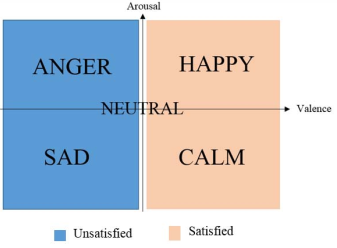
\includegraphics[angle=0, width=0.6\textwidth]{Figures/Satisfaction_from_VA.PNG}
  \caption{Satisfaction inference from VA values}
  \label{fig:SatisfactionFromVA}
  \end{center}
\end{figure}

The FaceReader product of the company Noldus\cite{Noldus:2020:Facereader} makes use of the seven basic emotions ,like happy or angry, and convert them into values for valence and arousal.

In a survey conducted in 2006 \cite{Poirier:2016:AdsFacialExpression}, the authors measured the effectiveness of ads through facial expressions.
\begin{quote}
    emotional journey, which relates to the positive or negative emotional variation  (valence between -1 and 1 where -1: 100\% negative expression, 1: 100\% positive expression and 0: neutral expression), remains the most powerful predictor of ad appreciation 
\end{quote}

\section{Value Co-Creation}
The co-creation of value is a core concept inside the Service-Dominant Logic (S-D Logic) that every client interaction can be described as a service. In this logic, the service's value is co-created by experiences between the service provider and the service user.\cite{Payne:2008:ValueCo-Creation}
\newline\newline
In comparison to S-D Logic where value is embedded in experiences, in the 'traditional' Goods-Dominant Logic (G-D Logic) value is embedded in goods and thus is only created by the produce of goods, but not by the user/client. \cite{Payne:2008:ValueCo-Creation}
\newline\newline
As a result, S-D Logic places the client at the same level of companies as the co-creator of value. As both of them engage in dialog through the product design and delivery stage, thus co-creating value through customized products. This co-creation can take place, for example, through the emotional engagement of the customer, as well as the co-design of product or even the transfer of labor to the customer (e.g. IKEA products). \cite{Payne:2008:ValueCo-Creation}
\newline\newline
\textbf{How does value co-creation manifest itself in this thesis?}